\documentclass[10pt,journal,compsoc]{IEEEtran}
\newif\ifpeerreview

%%% Important: for camera ready submissions, replace the following line
%%% with \peerreviewfalse
\peerreviewfalse


\usepackage[nocompress]{cite}
\usepackage{url}
\usepackage{amsmath,amssymb,graphicx}
\usepackage{hyperref}
\usepackage{float}
\usepackage{gensymb}
\usepackage{algorithm}
\usepackage{algpseudocode}

\usepackage{lipsum} % Only used to generate random text.


\usepackage[switch]{lineno}

% Insert your paper ID and information below
\newcommand{\paperID}{XXXX}

% Enter your paper title below
\title{CSC494 Project Report}

% Enter your author information before
% Note this is only necessary for the camera review. Submissions are anonymized.
\author{Yuezhexuan(Jason) Zhu}


\begin{document}


% Make Title
\ifpeerreview
\linenumbers \linenumbersep 15pt\relax 
\author{Paper ID \paperID\IEEEcompsocitemizethanks{\IEEEcompsocthanksitem This paper is under review for ICCP 2020 and the PAMI special issue on computational photography. Do not distribute.}}
\markboth{Anonymous ICCP 2020 submission ID \paperID}%
{}
\fi
\maketitle


% The first section title should be wrapped inside a \IEEEraisesectionheading as follows.
\IEEEraisesectionheading{
  \section{Introduction}\label{sec:introduction}
}
\IEEEPARstart{T}{his} CSC494 project is inspired by the paper "holocurtain"\cite{holocurtain}. Its core mechanism is to construct a highly-programmable and light-efficient structured light solution with high frame rate, which is called "binary holography". By combining binary holography with rolling-shutter camera, the programmable light curtain, holocuratin, is constructed.

This semester, mentored by Esther Lin, I aim at using similar set of laser source and \hyperref[sec:2.1]{digital micromirror device (DMD)} to replicate binary holography. While the replication is not completed this term and I'll continue on next term, I've worked on these subjects:
\begin{enumerate}
    \item Code Implementation - I programmed the modified Gerchberg-Saxton (GS) algorithm introduced in the paper\cite{holocurtain} that calculates the pattern of the binary holography, more detail in \hyperref[sec:3.1]{section 3.1} and \hyperref[sec:4.2]{section 4.2}. I also implemented tool for converting normal images into ideal DMD input format.
    \item Imaging Device Control Analysis - I probed into both the physical alignment and the software control of the imaging devices DMD and lens. Details of DMD control is in \hyperref[sec:3.2]{section 3.2} and \hyperref[sec:user_guide]{appendix}.
    \item Experiment Setup - I analyzed the DMD and got familiar with its control software, then worked on CAD design for crafting the frame that fix the DMD device. CAD modeling details inside \hyperref[sec:4.1]{section 4.1}.
    \item Theory Learning and Laser Training - I learned ray optics, wave optics, and fourier optics to help me understand the theorem behind the mechanism of holocurtain, and took laser safety training to get the qualification to work in the lab. I've listed textbook details in \hyperref[sec:2.1]{section 2.1}.
\end{enumerate}

In this report, I'll elaborate on the results I've made in the aforementioned sections. You can also check my work traces and all materials at the \href{https://github.com/zhuyuezx/CSC494_holoprojector/tree/main}{github repository for this project}.

\section{Related Work}
\label{sec:Related Work}

\subsection{Textbooks I Referred to}
\label{sec:2.1}
There are three textbooks recommended by Esther from which I learned the basics of electromagnetism and the fourier optics that explains the mechanism behind holocurtain. Some notes can be accessed on \href{https://github.com/zhuyuezx/CSC494_holoprojector/tree/main/Notes}{notes folder on github}.

Classical and Modern Optics\cite{ray optics} - I learned paraxial rays approximation and the modeling of composite optical systems using linear algebra.

Introduction to Electrodynamics\cite{electrodynamics} - This textbook helps to have a basic understanding of the electromagnetism. To be specific, I got familiar with the complex form of wave equation, the concept of plane wave, and the interference of plane waves throughout the learning, which helped me better with understanding the fourier optics.

Introduction to Fourier Optics\cite{fourier optics} - Thanks to this textbook, I assembled the scattered pieces of fourier transform knowledge into a general concept, and got the sense of the connection between lens and fourier transform. This is the core part that explains how holocurtain is formed, I will emphasize more in \hyperref[sec:2.4]{section 2.4}.
\begin{figure}[!h]
    \centering
    \includegraphics[width=0.4\textwidth]{img/note1.jpg}
    \caption{Note I took during learning}
\end{figure}

\subsection{Digital Micromirror Device (DMD)}
\label{sec:2.2}
 Digital Micromirror Device\cite{DMD}(DMD) is a type of optical micro-electrical-mechanical system (MEMS) featuring an array of highly reflective aluminum micromirrors. Each individual mirror, referred to as a pixel, is capable of tilting a small angle diagonally on two directions. For the make TI DLP670S used in this project, it has ±17.5 tilting degree.

\begin{figure}[!h]
    \centering
    \includegraphics[width=0.35\textwidth]{img/DMD.png}
    \caption{Illustration of how a micromirror functions, taken from TI documentation\cite{DMD}}
    \includegraphics[width=0.35\textwidth]{img/DMD2.png}
    \caption{Mechanical structure of the micromirror, taken from TI documentation\cite{DMD}}
\end{figure}

When the mirror has a positive degree, it's in the "on" state, and reflects the light towards projection lens. When it has a negative degree, it's in the "off" state and reflected light will be absorbed. 

DMD consists of millions of mirror pixels and each of the pixel can switch its state independently in over 10khz frame rate, which enables DMD to create any kind of pixelized bianry image. Then, utilizing light source that can alternate in primary colors and different exposure length in unit of time, DMD can convert arbitrary digital frames to structured light pattern in real world.

\subsection{Gerchberg-Saxton (GS) algorithm}
\label{sec:2.3}

The Gerchberg-Saxton (GS) algorith\cite{GS} is an iterative algorithm targeting at retrieving the phase of source wavefront given intensity measurements from two different planes. In normal case, two planes are the image plane and the far field diffraction plane. The ideal source phase distribution retrieved by GS algorithm would match the amplitude distribution of the target after applying fourier transform.

For the detail of the algorithm, starting with the random initialization of the source phase, the algorithm will perform the cycle which use the last step output for next step input: fourier transform $\rightarrow$ enforce target amplitude $\rightarrow$ inverse fourier transform $\rightarrow$ enforce source phase $\rightarrow$ fourier transform $\rightarrow$ ...

In the holocurtain paper and this project, the GS algorithm is modified for obtaining the ideal binary holography needed, please see \hyperref[sec:3.1]{section 3.1} for detail.

\subsection{Holocurtains}
\label{sec:2.4}

Figure\ref{fig:fig3} below shows the setup of the holocurtain paper, and it can be decomposed into three parts: 
\begin{enumerate}
    \item Using laser and DMD to create binary holography at fourier plane (fiber laser + Lens1 + fourier plane)
    \item Fourier transform with target shape formed at image plane (Lens2 + Knife Edge)
    \item The triangulation of target shape projection with rolling-shutter camera at figure\ref{fig:fig4} (objective lens + rolling-shutter camera)
\end{enumerate}
\begin{figure}[!h]
    \centering
    \includegraphics[width=0.45\textwidth]{img/holocurtain2.png}
    \caption{Setup of the holocurtain, taken from holocurtain paper\cite{holocurtain}}
    \label{fig:fig3}
\end{figure}
\begin{figure}[!h]
    \centering
    \includegraphics[width=0.45\textwidth]{img/holocurtain.png}
    \caption{Illustration of holocurtain, taken from holocurtain paper\cite{holocurtain}}
    \label{fig:fig4}
\end{figure}

I'll emphasize on several essential design decisions mentioned in the paper:
\begin{itemize}
    \item The reason of choosing binary holography:
    
    It can be best explained using the table taken from the paper:
    
    \begin{figure}[!h]
        \centering
        \includegraphics[width=0.5\textwidth]{img/holocurtain3.png}
        \caption{Table of comparisons between multiple solutions, taken from holocurtain paper\cite{holocurtain}}
        \label{fig:fig5}
    \end{figure}

    The binary holography created by part1 is light-efficient, has high frame rate, and has great programmability, making it the best solution
    \item Fourier optics applied in part2:
    
    With binary holography starting from the focus plane of lens2, it forms an interference pattern at the image plane that can be described using fourier transform. Let the original binary image be $u(x, y)$, with phase aberration of the DMD as $a(x, y)$, we can get the distribution at the image plane $U(s, t)$:
    \begin{equation}
        U(s, t) = \mathcal{F}\{u(x, y) \cdot a(x, y)\}(s, t)
    \end{equation}
    While it's binary pattern at fourier plane, it can approximate arbitary pattern after fourier transform.
    \item Missing coordination detail of the projector with rolling-shutter camera:
    
    For this part, the paper doesn't have a discussion about the coordinating the rolling-shutter camera with projected pattern, while I consider it an essential and tricky part for replication in the future.
\end{itemize}

Here are the types of the hardware used in holocurtain setup:
Coherent Sapphire LPX 530-300 Laser (laser source), DLP Lightcrafter 6500 EVM from Texas Instruments (DMD), UI-3240CP- NIR camera with 8mm f/1.4 lens (rolling-shutter camera).

\section{Method}
\label{sec:Method}

This section will focus on the methods I've applied in this project for holocurtain replication and experiment setup.

\subsection{Modified Gerchberg-Saxton(GS) Algorithm}
\label{sec:3.1}

For the normal case of GS algorithm, the algorithm takes observed amplitude from two planes - image plane and fourier plane, and use these two planes as the constraint. 

In this project, there's only one designated target fourier plane as the constraint, and the method manually adds the binary pattern constraint to the image plane for the second constraint. In addition, for better accuracy, the phase aberration introduced by DMD device, calling it $a(x, y)$, is considered, which can be recorded as an default value input in the algorithm.

\begin{figure}[!h]
    \centering
    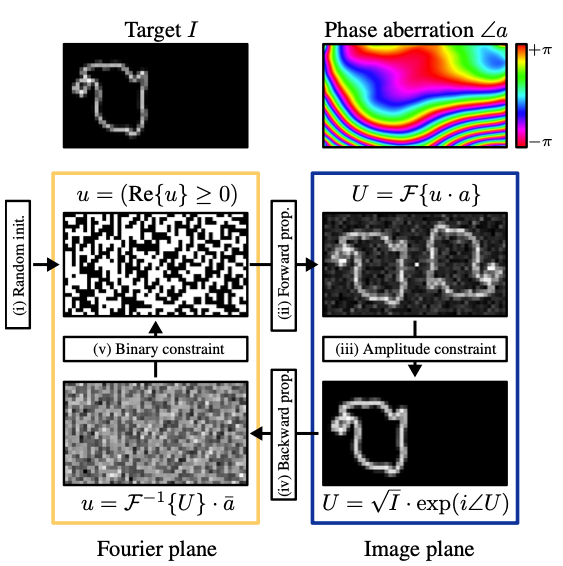
\includegraphics[width=0.5\textwidth]{img/GS_paper.jpg}
    \caption{Illustration of modified GS, taken from holocurtain paper\cite{holocurtain}}
    \label{fig:fig7}
\end{figure}

Therefore, staring with the random initialization of the binary pattern with size 2716$\times$1600 (Resolution of TI DLPC670S used in this project), calling it $u(x, y)$, the iterative steps of the modified GS algorithm are:
\begin{enumerate}
    \item Apply fourier Transform to the binary pattern
    $$U(s, t) = \mathcal{F}(u(x, y) \cdot a(x, y))$$
    \item Replace the amplitude of $U(s, t)$ with the amplitude of target $I(s, t)$ $$U(s, t) = \sqrt{I}\cdot exp(i\angle U)$$
    \item Apply inverse fourier transform 
    $$u(x, y) = \mathcal{F}(U(s, t))\overline{a(x, y)}$$
    \item Enforce binary constraint to $u(x, y)$
    $$u(x, y) = Re(u) \geq 0$$
\end{enumerate}

By iterating over these four steps, the modified GS algorithm converges quickly. With the modified GS algorithm ready, for an arbitrary 3D curtain, I can decompose it into frames of 2D shapes and calculate the corresponding batch of binary pattern. By playing these binary patterns repeatedly in high frame rate, the holocurtain is constructed. So, DMD controlling is the following essential point.

\subsection{DMD and controlling software analysis}
\label{sec:3.2}
Precise calibration is needed to make the DMD working as expected, after probing into details of the holocurtain experiment setup, I've concluded several rules for TI DLP670S used in the project. To avoid inaccuracy, x-axis refers to the axis along DMD surface horizontally; y-axis as the axis along DMD surface vertically; and z-axis as the one that pass through DMD surface:
\begin{itemize}
    \item x-y plane should be orthogonal to the motherboard
    \item The incoming laser beam should keep a 35\textdegree ($17.5 \times 2$\textdegree) angle with the x-y plane so the beam reflected out would be on the y-z plane.
    \item z-axis should keep a 45\textdegree angle with the motherboard to ensure that the reflected beam is on x-z plane. This is because each mirror unit tilts on its diagonal, resulting in such 45\textdegree adjustment
\end{itemize}

\begin{figure}[!h]
    \centering
    \includegraphics[width=0.5\textwidth]{img/software.png}
    \caption{GUI of the software}
    \label{fig:fig8}
\end{figure}

For the TI DLP670S I'm using in this project, TI provides a software for configuring input patterns and their sequence as shown in figure\ref{fig:fig8}. It shows status information about the device after connection, and provides interface for controlling the pattern displayed on the DMD.

In the pattern mode, the software takes a series of bmp files as input, and you can configure the sequence and length of the bmp images. After the edit, the sequence can be updated to the look-up table of DMD and displayed repeatedly.

\subsection{CAD-modeling-assisted experiment setup}
\label{sec:3.3}
It would be time-consuming if I build up the experiment without a clear global view since any mismatch would lead to potential complete restructure. So, I took advantage of the online cloud CAD tool Onshape for building up a digital design.

\subsubsection{DMD fixation}
DLP670S need to connect with its motherboard using two flexible cables to work normally, while there's no natural fixation provided. The plan is to fix the motherboard and DMD each on one side of the metal board, so I can then connect the metal board to the motherboard without worrying about strength of PCB.

So, I designed the middle board that contains four holes at corner for motherboard, four holes in central for DMD, and two holes for right angle fixation to breadboard. By assembling these three parts virtually, I can ensure that metal board design is reliable.

\begin{figure}[!h]
    \centering
    \includegraphics[width=0.5\textwidth]{img/CAD.png}
    \caption{Example of CAD design for fixation of DMD on breadboard}
    \label{fig:fig9}
\end{figure}

\subsubsection{Assembly of components on cloud}

For most of the components of the experiment like lens, they need to be fixed properly and precisely to function normally, while some have their own nodes for fixation, others requires precise alignment similar to DMD. 

So, the proposed method is to import CAD models of those components along with the right angle mounting adapters and screws into the cloud assembly given that most CAD models of components can be found at the official website. This helps me to have a clear concept of the overall setup, and then I can better arrange the step-by-step construction of experiment in the lab.

\subsubsection{Closure Setup}
A class 3B laser source is used in this project, so a complete closure is required to ensure there's no potential laser hazard outside the closure.

With the plan of building up opaque and fireproof material at the sides of the breadboard, CAD modeling can help me to test on multiple designs virtually so as to determine the final plan in real setup.

\section{Results}
\label{sec:Results}

\subsection{CAD models}
\label{sec:4.1}

Till the end of this semester, I've been working on DMD fixation and components assembling in the lab. For the closure setup, I'll continue on next semester. So, here are the CAD designs I've completed on Onshape:

\begin{figure}[!h]
    \centering
    \includegraphics[width=0.5\textwidth]{img/CAD2.png}
    \caption{Correspondence of design script with assembly}
    \label{fig:fig10}
\end{figure}

\subsection{GS-algorithm performance}
\label{sec:4.2}
\begin{figure*}[!h]
    \centering
    \includegraphics[width=0.9\textwidth]{img/result.png}
    \caption{Visual results of modified GS algorithm}
    \label{fig:fig11}
\end{figure*}

\begin{table}[!t]
\renewcommand{\arraystretch}{1.3}
\caption{Evaluation metrics for modified GS algorithm in figure\ref{fig:fig11}}
\centering
\begin{tabular}{c||c|c|c}
\hline
 & PSNR(dB) & SSIM & NRMSE\\
\hline\hline
Example & 23.27 & 0.86 & 0.07\\
\hline
Airforce Chart & 33.67 & 1.00 & 0.02\\
\hline
Simens Start & 15.25 & 0.91 & 0.17\\
\hline
\end{tabular}
\label{table:metrics}
\end{table}

I've implemented my version of the GS algorithm in python, and generated results on multiple aspects. First is the visual comparison in figure\ref{fig:fig11}. There are three samples selected: example from holocurtain paper, airforce chart, and simens start. Then, for visualization, it starts with the target pattern, following with binary pattern calculated from GS algorithm $\rightarrow$ fourier plane representing the absolute value after fourier transform $\rightarrow$ fourier plane after amplitude constraint $\rightarrow$ L1 difference between amplitude constraint result and target.

In addition to visual comparison, the evaluation metrics are listed in table\ref{table:metrics}. For relative simple, monochromatic patterns like the example and airforce chart, the algorithm can achieve a high score, while it doesn't have a perfect approximation with complex boundaries and various gray scale in Simens Start. This is because of the natural limitation of the binary pattern and resolution of DMD.

For this project, the results shows that this modified GS algorithm is sufficient for the replication of holocurtain.

\subsection{Experiment setup progress in the lab}
\label{sec:4.3}

Since I started on lab works at the beginning of November, I've focused on DMD analysis and its fixation, and here is the current progress on experiment setup:
\begin{figure}[!h]
    \centering
    \includegraphics[width=0.5\textwidth]{img/lab1.jpg}
    \caption{Current progress in the lab}
    \label{fig:fig12}
\end{figure}

I've been familiar with the DMD, and now working on the fixation on breadboard using AB90A. With the CAD design completed, my next is to craft the metal middle board with the help from Esther.

\section{Discussion}
\label{sec:Discussion}

\subsection{Limitation: Innovation beyond holocurtain}
The core mechanism of holocurtain\cite{holocurtain} is the binary-holography generator powered by DMD, while rolling-shutter camera is like the add-on. So, with the binary-holography generator replicated, it can incorporate with other imaging devices that will extend its potentials.

\subsection{Bottleneck: redesign due to device discrepancy}

The discrepancies of DMD and lens between holocurtain project and this project is a bottleneck for evaluating whether the replication reaches the expected effect. For instance, the layout of DLPC900 and DLP670S has relative difference, resulting in different fixation plan, which further influence the overall setup. Considering that for most cases one cannot get the exact components for replication, device discrepancy is a genuine bottleneck.

\subsection{Bottleneck: Calibration of device}
The holocurtain paper\cite{holocurtain} doesn't emphasize on how phase aberration is measured, and how to coordinate rolling-shutter camera with holography projector, while these details would be crucial for my setup in the lab. Therefore, it will induce extra workload for figuring out the method and applying calibration in future stages of this project.

\subsection{Plan for next semester}

Based on discussion with Esther and approval from professors, I'll continue my work on this project next semester, and here are the rough goals:
\begin{enumerate}
    \item Set up the complete laser propagation route on optical breadboard that can project structured light. This includes fixing DMD, mounting lens, aligning the laser propagation route, and construct the laser closure.
    \item Define the 3D testing surface, like bunny, calculate the frames of its 2D intersections, and then transform them into binary patterns that can be accepted by DMD API.
    \item Measure required data for device calibration and then perform calibration.
    \item Read paper and gather potential ideas beyond holocurtain.
\end{enumerate}

\section*{Code}
\label{sec:Code}

All code and materials can be found at the \href{https://github.com/zhuyuezx/CSC494_holoprojector}{github repository} for this project\footnote{link: https://github.com/zhuyuezx/CSC494\_holoprojector}, and here is the pseudo-code for modified GS algorithm:
\begin{algorithm}
\caption{Modified GS algorithm}\label{alg:cap}
\begin{algorithmic}[1]
\State \textbf{Let}:
    \State fft2 - fast fourier transform 2D
    \State inv\_fft2 - inverse fast fourier transform 2D
    \State target - the target shape, 2D array of 8 bit value
    \State abr - aberration of DMD device predefined
\State
\State \textbf{algorithm} GS(target, iter, abr) is:
\State h, w $\gets$ target.shape
\State u $\gets$ rand(h, w) $\geq 0.5$ \Comment{\textit{Step1: random init}}
\For {\_ in range(iter)}
    \State u $\gets$ fft2($u \cdot abr$) \Comment{\textit{Step2: forward propagation}}
    \State u $\gets$ sqrt(target) $\cdot$ exp($1j \cdot \angle u$) \Comment{\textit{Step3: Amplitude Constraint}}
    \State u $\gets$ inv\_fft2($u \cdot \overline{abr}$) \Comment{\textit{Step4: Backward Propagation}}
    \State u $\gets$ real(u) $geq 0$ \Comment{\textit{Step5: Binary Constraint}}
\EndFor
\State
\State \textbf{return} u
\end{algorithmic}
\end{algorithm}

% Any acknowledgments to only be included in camera ready
\ifpeerreview \else
\section*{Acknowledgments}

I want to give great thanks to my CSC494 mentor Esther Lin. She gives me instruction and insights on how to work on this project academically, and helped me on every aspect, especially paper reading and experiment setup. 

I want to give great thanks to Professor Kyros Kutulakos and Professor David Lindell, for helping me with managerial things of the project in lab and giving out suggestions in general direction.

I also want to thank Mian Wei, the lab manager, for offering me a lab etiquette tutorial and discussed closure setup in lab together with professor Kyros.



\fi

\bibliographystyle{IEEEtran}

{
\small
\bibliographystyle{plain}
\begin{thebibliography}{9}
\bibitem{holocurtain}
Chan, Dorian and Narasimhan, Srinivas and O'Toole (2022) Matthew Holocurtains: Programming Light Curtains via Binary Holography
\bibitem{ray optics}
Daniel A. Steck (2021). Classical and Modern Optics. 
\bibitem{electrodynamics}
Griffiths, D. J. (2024). Introduction to electrodynamics. Cambridge University Press. 
\bibitem{fourier optics}
Goodman, J. W. (1996). Introduction to fourier optics. McGraw-Hill. 
\bibitem{DMD}
Introduction to ±12 degree orthogonal digital micromirror ... - analog. (n.d.). https://www.ti.com/lit/an/dlpa008b/dlpa008b.pdf 
\bibitem{GS}
 Gerchberg, R. W.; Saxton, W. O. (1972). "A practical algorithm for the determination of the phase from image and diffraction plane pictures" (PDF). Optik. 35: 237–246.
\end{thebibliography}
}

\newpage 

\appendix

\section{Appendix}

\section*{Brief DMD User Guide}
\label{sec:user_guide}
The content is mostly from the offical \href{https://www.ti.com/lit/pdf/dlpu101}{user guide of DLPC900 from Texas Instrument}, combing with my personal experience.
\begin{figure}[!h]
    \centering
    \includegraphics[width=0.5\textwidth]{img/ports.png}
    \caption{Connectors of DLPC900 (motherboard)}
    \label{fig:fig13}
\end{figure}

\begin{itemize}
    \item J8 – host USB input
    \item J20 - 12V DC power input
    \item J18, J19 – DMD connector
    \item D5 – FPGA init done
    \item D7 – Green Heartbeat LED (When toggling indicates Primary DLPC900 controller is operating)
    \item D11 – 12V power LED
\end{itemize}

\begin{figure}[!h]
    \centering
    \includegraphics[width=0.5\textwidth]{img/DMD3.png}
    \caption{Complete device after being assembled}
    \label{fig:fig14}
\end{figure}
External Power supply requirement: 12V DC, Minimum Current: 0A, maximum current: 7A, inner Diameter: 2.5mm, outer diameter: 5.5mm

USB cable requirement: A to B usb cable

Here are the procedures for powering DMD and controlling it to show patterns using software:
\begin{enumerate}
    \item Connect a 12-V DC power supply to J20, and you should see D5, D11, and D12 light up with D7 and D9 toggling on and off after 5 seconds of initialization.
    \item Open the contorl software (you can download it \href{https://www.ti.com/tool/DLPLCRC900DEVM}{here}\footnote{link: https://www.ti.com/tool/DLPLCRC900DEVM}) and connect the usb cable to J8 portal. You should see green signal inside "System Control" section in software's top-left region.
    \item Change the operation mode from "video mode" to "pattern-on-the-fly" mode in the "Operation Mode" section at fourth left panel from top. Then, switch to "Pattern Mode" at the top panel.
    \item Click the "Add pattern" button (the one inside "menu section" with file+ icon), and the default patterns can be found at C: \textbackslash Texas Instruments-DLP \textbackslash DLPC900REF-SW-5.x \textbackslash DLPC900REF-GUI \textbackslash Images and Batch files \textbackslash [DMD]\_Images, Or use the path where you store you patterns.
    \item In the left panel inside, you can control the exposure time, dark time, depth, and color of each pattern by selecting them. In the right panel inside. For example, the interface would be like this:
    \begin{figure}[!h]
    \centering
    \includegraphics[width=0.5\textwidth]{img/software2.png}
    \label{fig:fig15}
    \end{figure}
    \item Click "Update LUT" to update the look up table of DMD, and then click start. At this time, you should see patterns showing on the DMD. To have a easy observation, you need to set a large exposure time as it uses microsecond(us) for time unit.
    \item To observe the patter, I recommend to use torchlight and cast ray in around 35\textdegree angle and adjust the position to make the reflection on screen or wall, where you can observe the change it pattern in low resolution as the incoming lights are not calibrated.
\end{enumerate}

\end{document}